\documentclass{article}


\usepackage[margin=0.6in]{geometry}
\usepackage{amssymb, amsmath, amsfonts}
\usepackage{mathtools}
\usepackage{physics}
\usepackage{placeins}
\usepackage{enumerate}
\usepackage{cancel}
\usepackage{array}
\usepackage{color}
\newcommand{\Rl}{\mathbb{R}}
\newcommand{\prob}{\mathbb{P}}
\newcommand{\cov}{\text{cov}}
\newcommand{\vari}{\text{var}}
\newcommand{\cor}{\text{cor}}
\newcommand{\expec}{\mathbb{E}}
\newcommand{\f}[3]{#1\ :\ #2 \rightarrow #3}

\title{PBG 200A Notes}
\author{Sam Fleischer}
\date{October 31, 2016}

\begin{document}
    \maketitle

    \section{Questions from the Notes}
        \subsubsection*{Question 1}
            \begin{align}
                H_t &= H_0\exp(-\frac{t}{2N}) \\
                0.0049 &= 0.005\exp(-\frac{200/3}{2N}) \\
                \ln0.98 &= -\frac{200}{6N} \\
                N &= -\frac{200}{6\ln0.98} \\
                N &= 1650
            \end{align}
        \subsubsection*{Question 2}
            $x = 0.5$:
            \begin{figure}[ht!]
                \centering
                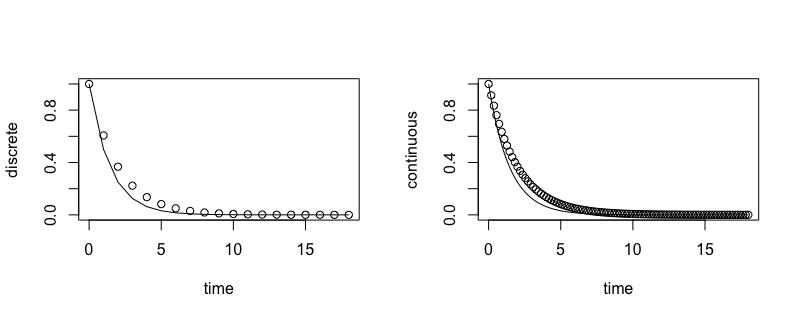
\includegraphics[scale=0.4]{fig1.png}\\
            \end{figure}
            \FloatBarrier
            $x = 0.1$:
            \begin{figure}[ht!]
                \centering
                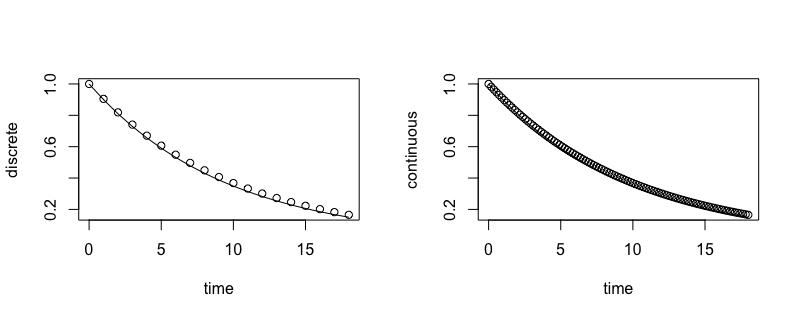
\includegraphics[scale=0.4]{fig2.png}\\
            \end{figure}
            \FloatBarrier
            $x = 0.01$:
            \begin{figure}[ht!]
                \centering
                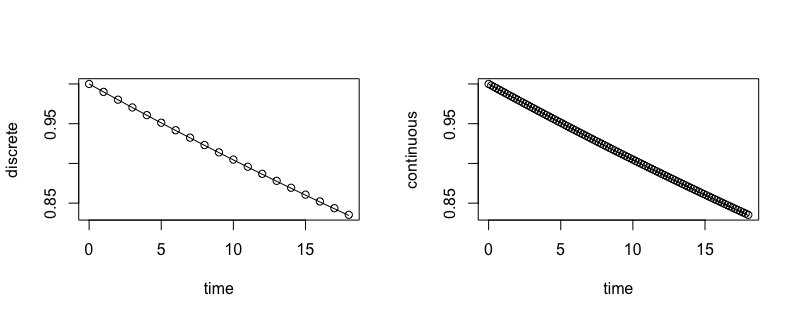
\includegraphics[scale=0.4]{fig3.png}\\
            \end{figure}
            \FloatBarrier

        \subsubsection*{Question 3}
            \begin{enumerate}[\bf\ \ A)]
                \item $\pi_1 = 0.0012$, $\pi_2 = 0.000014$ ?????
                \item $N_i = \frac{\theta_i}{4\mu}$ for $i = 1,2$.  If $\mu = 2\times10^{-8}$ and $\theta_1 = 0.0012$, then $N_1 = 15,000$.  If $\theta_2 = 0.000014$, then $N_2 = 175$.
                \item Oh my God they're adorable.
            \end{enumerate}

\end{document}















